\documentclass[a4paper,12pt,titlepage]{article}
\usepackage{amsmath} 
\usepackage{amssymb}
\usepackage[nottoc]{tocbibind}
\usepackage{float}
\usepackage{indentfirst}
\author{\textit{Jiang Yicheng}\\\textit{515370910224}}
\title{\textbf{VV286\\ Honors Mathematics IV\\
Ordinary Differential Equations\\
		Assignment 4}}
\date{\today}
\usepackage{extarrows}
\usepackage{mathrsfs}
\usepackage{dsfont}
\usepackage[top=1 in, bottom=0.8 in, left= 1in, right=1 in]{geometry}
\usepackage{fancyhdr,lastpage}
	\pagestyle{fancy}
	\fancyhf{}
\cfoot{Page \thepage\ of \pageref{LastPage}}
\usepackage{multirow}
\usepackage{gauss}
\usepackage{geometry}
\usepackage{graphicx}
\begin{document}

\maketitle

\section*{Exercise 4.1}
\begin{align*}
&(A-3\mathds{1})v=\left(\begin{array}{cccc}
4-3&-4&-11&11\\
3&-12-3&-42&42\\
-2&12&37-3&-34\\
-1&7&20&-17-3
\end{array}\right)\left(\begin{array}{c}
v_1\\
v_2\\
v_3\\
v_4
\end{array}\right)=\left(\begin{array}{c}
0\\
0\\
0\\
0
\end{array}\right)\\
\Rightarrow& \left(\begin{array}{cccc}
1&-4&-11&11\\
3&-15&-42&42\\
-2&12&34&-34\\
-1&7&20&-20
\end{array}\right)\left(\begin{array}{c}
v_1\\
v_2\\
v_3\\
v_4
\end{array}\right)=\left(\begin{array}{c}
0\\
0\\
0\\
0
\end{array}\right)\Rightarrow v_1=v_4-v_3\wedge v_2=3v_4-3v_3\\
\Rightarrow& v=\left(\begin{array}{c}
v_4-v_3\\
3v_4-3v_3\\
v_3\\
v_4
\end{array}\right)=v_3\left(\begin{array}{c}
-1\\
-3\\
1\\
0
\end{array}\right)+v_4\left(\begin{array}{c}
1\\
3\\
0\\
1
\end{array}\right)
\end{align*}
So we can find two independent eigenvectors by choosing
$$v_1=\left(\begin{array}{c}
-1\\
-3\\
1\\
0
\end{array}\right),\,\,\,\,\,\,\,\,\,\,\,\,\,\,v_2=\left(\begin{array}{c}
1\\
3\\
0\\
1
\end{array}\right)$$
Hence, $dimV_{\lambda} = 2$ and we need to find two generalized eigenvectors. $m=a_{\lambda}-dimV_{\lambda}+1=4-2+1=3$. We can find that

$$(A-3\mathds{1})^2=\left(\begin{array}{cccc}
0&1&3&-3\\
0&3&9&-9\\
0&-2&-6&6\\
0&-1&-3&3
\end{array}\right),(A-3\mathds{1})^3=\left(\begin{array}{cccc}
0&0&0&0\\
0&0&0&0\\
0&0&0&0\\
0&0&0&0
\end{array}\right)$$

We see that any vector solves $(A - 3\mathds{1})^3v = 0$ , and we can easily choose a vector such that $(A - 3\mathds{1})^2v  \neq 0$. 

So we can set
$$v^{(3)}=\left(\begin{array}{c}
4\\
1\\
0\\
0
\end{array}\right),v^{(2)}=(A-3\mathds{1})v^{(3)}=\left(\begin{array}{c}
0\\
-3\\
4\\
3
\end{array}\right),v^{(1)}=(A-3\mathds{1})v^{(2)}=\left(\begin{array}{c}
1\\
3\\
-2\\
-1
\end{array}\right)=-2v_1-v_2$$
Then we set $U=(v_1,v^{(1)},v^{(2)},v^{(3)})$ and we can get that
$$U^{-1}AU=\left(\begin{array}{cccc}
3&0&0&0\\
0&3&1&0\\
0&0&3&1\\
0&0&0&3
\end{array}\right)$$
and a basis of generalized eigenvectors is $\lbrace\left(\begin{array}{c}
-1\\
-3\\
1\\
0
\end{array}\right),\left(\begin{array}{c}
1\\
3\\
-2\\
-1
\end{array}\right),\left(\begin{array}{c}
0\\
-3\\
4\\
3
\end{array}\right),\left(\begin{array}{c}
4\\
1\\
0\\
0
\end{array}\right)\rbrace$. 

\section*{Exercise 4.2}
Since $F:\mathbb{R}^2\mapsto \mathbb{R}^2$ is a constant linear force field, then we can consider it as a matrix in $2\times 2$, i.e.
$$F(x_1,x_2)=Fx$$
where $x=\begin{pmatrix}
x_1\\
x_2
\end{pmatrix}
$. According to Newton's second law, sicne the mass of particle is $m=1$,
$$F(x_1,x_2)=ma=v'$$
where $v'=a$ is the acceleration of the particle and $v=\begin{pmatrix}
v_1\\
v_2
\end{pmatrix}$ is the velocity of it. Moreover, according to the definition of velocity, we know  that
$$v=x'$$ 
so
$$\begin{pmatrix}
x'\\
v'
\end{pmatrix}=\begin{pmatrix}
v\\
Fx\\
\end{pmatrix}=\begin{pmatrix}
0&\mathds{1}\\
F&0
\end{pmatrix}\begin{pmatrix}
x\\
v\\
\end{pmatrix}$$

For $F=\begin{pmatrix}
0&1\\
1&0
\end{pmatrix}$, set $A=\begin{pmatrix}
0&0&1&0\\
0&0&0&1\\
0&1&0&0\\
1&0&0&0
\end{pmatrix}$, then
$det(A-\lambda\mathds{1})=0\Leftrightarrow\lambda=\pm1,\pm i$.
\begin{enumerate}
\item $(A-\lambda)v=0\Leftrightarrow v_1=v_2=v_3=v_4$, so we choose $u_1=\begin{pmatrix}
1\\
1\\
1\\
1
\end{pmatrix}$
\item $(A+\lambda)v=0\Leftrightarrow v_1=v_2=-v_3=-v_4$, so we choose $u_2=\begin{pmatrix}
1\\
1\\
-1\\
-1
\end{pmatrix}$
\item $(A-i\lambda)v=0\Leftrightarrow v_2=-v_1\wedge v_3=iv_1\wedge v_4=-iv_1$, so we choose $u_3=\begin{pmatrix}
1\\
-1\\
i\\
-i
\end{pmatrix}$
\item $(A+i\lambda)v=0\Leftrightarrow v_2=-v_1\wedge v_3=-iv_1\wedge v_4=iv_1$, so we choose $u_4=\begin{pmatrix}
1\\
-1\\
-i\\
i
\end{pmatrix}$

\end{enumerate}
So $A$ is diagonalizable and the fundamental system is
$$\mathscr{F}=\lbrace e^t\begin{pmatrix}
1\\
1\\
1\\
1
\end{pmatrix},e^{-t}\begin{pmatrix}
1\\
1\\
-1\\
-1
\end{pmatrix},e^{it}\begin{pmatrix}
1\\
-1\\
i\\
-i
\end{pmatrix},e^{-it}\begin{pmatrix}
1\\
-1\\
-i\\
i
\end{pmatrix}\rbrace$$

So general solution for the system of equations is
$$\begin{pmatrix}
x_1(t)\\
x_2(t)\\
v_1(t)\\
v_2(t)
\end{pmatrix}=Re\begin{pmatrix}
c_1e^t+c_2e^{-t}+c_3e^{it}+c_4e^{-it}\\
c_1e^t+c_2e^{-t}-c_3e^{it}-c_4e^{-it}\\
c_1e^t-c_2e^{-t}+ic_3e^{it}-ic_4e^{-it}\\
c_1e^t-c_2e^{-t}-ic_3e^{it}+ic_4e^{-it}
\end{pmatrix}=\begin{pmatrix}
c_1e^t+c_2e^{-t}+c_5cost\\
c_1e^t+c_2e^{-t}-c_5cost\\
c_1e^t-c_2e^{-t}-c_5sint\\
c_1e^t-c_2e^{-t}+c_5sint
\end{pmatrix}$$
where $c_1,c_2,c_3,c_4,c_5\in\mathbb{R}$ are constant.

\section*{Exercise 4.3}

\begin{figure}[H]
    \centering
    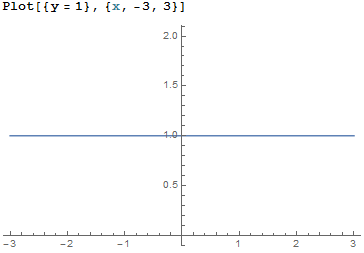
\includegraphics[width=8cm]{1.png}
\end{figure}
\subsection*{i)}
Set the acceleration of each mass is $a_1,a_2,a_3$, then $a_1=\ddot{d_1},a_2=\ddot{d_2},a_3=\ddot{d_3}$. Then according to laws of Newton and Hooke, we get that:
$$ma_1=F_1=k(d_2-d_1),ma_3=F_2=k(d_2-d_3),ma_2=-F_1-F_2=k(d_1-d_2-d_2+d_3) $$
So
$$\ddot{d}=\begin{pmatrix}
\ddot{d_1}\\
\ddot{d_2}\\
\ddot{d_3}
\end{pmatrix}=\dfrac{k}{m}\begin{pmatrix}
d_2-d_1\\
d_1-2d_2+d_3\\
d_2-d_3
\end{pmatrix}=\dfrac{k}{m}\begin{pmatrix}
-1&1&0\\
1&-2&1\\
0&1&-1
\end{pmatrix}\begin{pmatrix}
d_1\\
d_2\\
d_3
\end{pmatrix}=Ad$$

So $\ddot{d}=Ad$
\subsection*{ii)}
Set the velocity of mass is $v_1,v_2,v_3$, then $v_1=\dot{d_1},v_2=\dot{d_2},v_3=\dot{d_3}$. Then
\begin{align*}
\begin{pmatrix}
\dot{v}\\
\dot{d}
\end{pmatrix}=\begin{pmatrix}
\dot{v_1}\\
\dot{v_2}\\
\dot{v_3}\\
\dot{d_1}\\
\dot{d_2}\\
\dot{d_3}
\end{pmatrix}=\begin{pmatrix}
\ddot{d_1}\\
\ddot{d_2}\\
\ddot{d_3}\\
v_1\\
v_2\\
v_3
\end{pmatrix}=\begin{pmatrix}
\dfrac{k}{m}(d_2-d_1)\\
\dfrac{k}{m}(d_1-2d_2+d_3)\\
\dfrac{k}{m}(d_2-d_3)\\
v_1\\
v_2\\
v_3
\end{pmatrix}=\begin{pmatrix}
0&0&0&-\dfrac{k}{m}&\dfrac{k}{m}&0\\
0&0&0&\dfrac{k}{m}&-\dfrac{2k}{m}&\dfrac{k}{m}\\
0&0&0&0&\dfrac{k}{m}&-\dfrac{k}{m}\\
1&0&0&0&0&0\\
0&1&0&0&0&0\\
0&0&1&0&0&0
\end{pmatrix}\begin{pmatrix}
v_1\\
v_2\\
v_3\\
d_1\\
d_2\\
d_3
\end{pmatrix}
\end{align*}
So let $B=\begin{pmatrix}
0&0&0&-\dfrac{k}{m}&\dfrac{k}{m}&0\\
0&0&0&\dfrac{k}{m}&-\dfrac{2k}{m}&\dfrac{k}{m}\\
0&0&0&0&\dfrac{k}{m}&-\dfrac{k}{m}\\
1&0&0&0&0&0\\
0&1&0&0&0&0\\
0&0&1&0&0&0
\end{pmatrix}$ and then $\begin{pmatrix}
\dot{v}\\
\dot{d}
\end{pmatrix}=B\begin{pmatrix}
v\\
d
\end{pmatrix}$.

\subsection*{iii)}
When $k=m=1$, $B=\begin{pmatrix}
0&0&0&-1&1&0\\
0&0&0&1&-2&1\\
0&0&0&0&1&-1\\
1&0&0&0&0&0\\
0&1&0&0&0&0\\
0&0&1&0&0&0
\end{pmatrix}$
\begin{figure}[H]
    \centering
    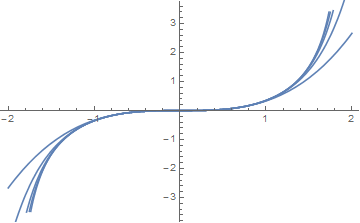
\includegraphics[width=14cm]{2.png}
\end{figure}
So eigenvalues of $B$ are $\lambda_1=\sqrt{3}i,\lambda_2=-\sqrt{3}i,\lambda_3=i,\lambda_4=-i,\lambda_5=0$ and eigenvectors are
$v_1=a_1\begin{pmatrix}
\sqrt{3}\\
-2\sqrt{3}\\
\sqrt{3}\\
-i\\
2i\\
-i
\end{pmatrix},v_2=a_2\begin{pmatrix}
\sqrt{3}\\
-2\sqrt{3}\\
\sqrt{3}\\
i\\
-2i\\
i
\end{pmatrix},v_3=a_3\begin{pmatrix}
1\\
0\\
-1\\
-i\\
0\\
i
\end{pmatrix},v_4=a_4\begin{pmatrix}
1\\
0\\
-1\\
i\\
0\\
-i
\end{pmatrix},v_5=a_5\begin{pmatrix}
0\\
0\\
0\\
1\\
1\\
1
\end{pmatrix}$ where $a_1,a_2,a_3,a_4,a_5\in\mathbb{C}\setminus\lbrace0\rbrace$.

\begin{figure}[H]
    \centering
    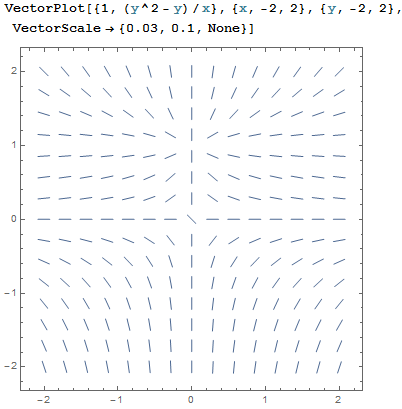
\includegraphics[width=14cm]{3.png}
\end{figure}

So the Jordan normal form $J$ of $B$ is $J=\begin{pmatrix}
0 &1& i&-i & -\sqrt{3}i&\sqrt{3}i\\
0 &1& 0& 0 &2\sqrt{3}i&-2\sqrt{3}i\\
0 &1&-i& i & -\sqrt{3}i&\sqrt{3}i\\
1 &0&-1&-1 &1&1\\
1 &0& 0& 0 &-2&-2\\
1 &0& 1& 1 &1&1
\end{pmatrix}$ and the matrix $S$ such that $B=SJS^{-1}$ is $S=\begin{pmatrix}
0&1&0&0&0&0\\
0&0&0&0&0&0\\
0&0&-i&0&0&0\\
0&0&0&i&0&0\\
0&0&0&0&-\sqrt{3}i&0\\
0&0&0&0&0&\sqrt{3}i
\end{pmatrix}$. 
\subsection*{iv)} 
\begin{figure}[H]
    \centering
    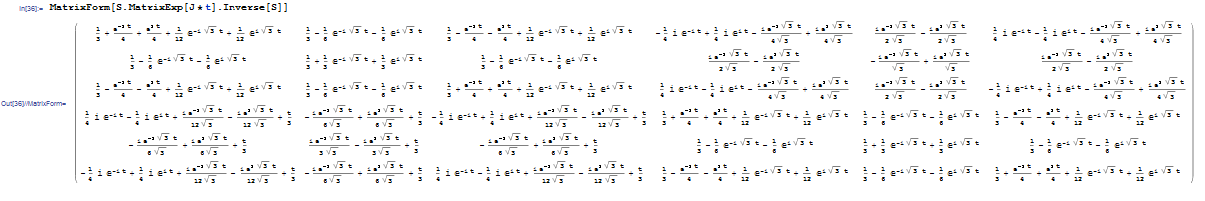
\includegraphics[width=15cm]{4.png}
\end{figure}
So $\Phi(t)=e^{Bt}=Se^{Jt}S^{-1}=$
\tiny
\begin{align*}
\dfrac{1}{6}\begin{pmatrix}
2+3cost+cos\sqrt{3}t&2-2cos\sqrt{3}t&2-3cost+cos\sqrt{3}t&-3sint-\sqrt{3}sin\sqrt{3}t&2\sqrt{3}sin\sqrt{3}t&3sint-\sqrt{3}sin\sqrt{3}t\\
2-2cos\sqrt{3}t&2+4cos\sqrt{3}t&2-2cos\sqrt{3}t&2\sqrt{3}sin\sqrt{3}t&-4\sqrt{3}sin\sqrt{3}t&2\sqrt{3}sin\sqrt{3}t\\
2-3cost+cos\sqrt{3}t&2-2cos\sqrt{3}t&2+3cost+cos\sqrt{3}t&3sint-\sqrt{3}sin\sqrt{3}t&2\sqrt{3}sin\sqrt{3}t&-3sint-\sqrt{3}sin\sqrt{3}t\\
3sint+\dfrac{1}{\sqrt{3}}sin\sqrt{3}t+2t&-\dfrac{2}{\sqrt{3}}sin\sqrt{3}t+2t&3sint+\dfrac{1}{\sqrt{3}}sin\sqrt{3}t+2t&2+3cost+cos\sqrt{3}t&2-2cos\sqrt{3}t&2-3cost+cos\sqrt{3}t\\
-\dfrac{2}{\sqrt{3}}sin\sqrt{3}t+2t&\dfrac{4}{\sqrt{3}}sin\sqrt{3}t+2t&-\dfrac{2}{\sqrt{3}}sin\sqrt{3}t+2t&2-2cos\sqrt{3}t&2+4cos\sqrt{3}t&2-2cos\sqrt{3}t\\
-3sint-\dfrac{1}{\sqrt{3}}sin\sqrt{3}t+2t&-\dfrac{2}{\sqrt{3}}sin\sqrt{3}t+2t&3sint+\dfrac{1}{\sqrt{3}}sin\sqrt{3}t+2t&2-3cost+cos\sqrt{3}t&2-2cos\sqrt{3}t&2+3cost+cos\sqrt{3}t\\
\end{pmatrix}
\end{align*}
\normalsize
So $\Phi(0)=\dfrac{1}{6}\begin{pmatrix}
2+3+1&2-2&2-3+1&0&0&0\\
2-2&2+4&2-2&0&0&0\\
2-3+1&2-2&2+3+1&0&0&0\\
0&0&0&2+3+1&2-2&2-3+1\\
0&0&0&2-2&2+4&2-2\\
0&0&0&2-3+1&2-2&2+3+1
\end{pmatrix}=\mathds{1}$.
\subsection*{v)}
\begin{figure}[H]
    \centering
    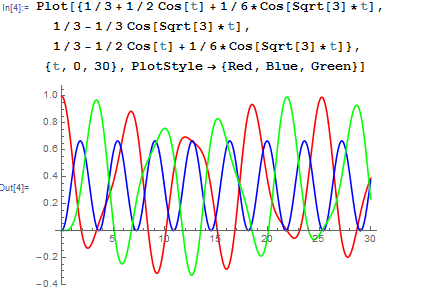
\includegraphics[width=11
    cm]{51.png}
    \caption{Figure for $v_1(t)=\dfrac{1}{3}+\dfrac{1}{2}cost+\dfrac{1}{6}cos\sqrt{3}t,v_2=\dfrac{1}{3}-\dfrac{1}{3}cos\sqrt{3}t,v_3(t)=\dfrac{1}{3}-\dfrac{1}{2}cost+\dfrac{1}{6}cos\sqrt{3}t$,red for $v_1(t)$, blue for $v_2$, green for $v_3$.}
\end{figure}

\begin{figure}[H]
    \centering
    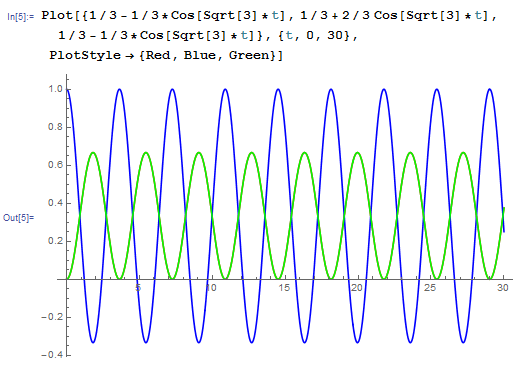
\includegraphics[width=11
    cm]{52.png}
    \caption{Figure for $v_1(t)=\dfrac{1}{3}-\dfrac{1}{3}cos\sqrt{3}t,v_2=\dfrac{1}{3}+\dfrac{1}{3}cos\sqrt{3}t,v_3(t)=\dfrac{1}{3}-\dfrac{1}{3}cos\sqrt{3}t$,red for $v_1(t)$, blue for $v_2$, green for $v_3$.}
\end{figure}

\begin{figure}[H]
    \centering
    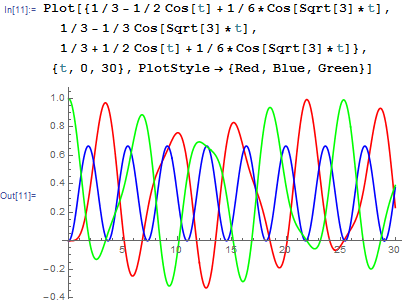
\includegraphics[width=11
    cm]{53.png}
    \caption{Figure for $v_3
    (t)=\dfrac{1}{3}+\dfrac{1}{2}cost+\dfrac{1}{6}cos\sqrt{3}t,v_2=\dfrac{1}{3}-\dfrac{1}{3}cos\sqrt{3}t,v_1(t)=\dfrac{1}{3}-\dfrac{1}{2}cost+\dfrac{1}{6}cos\sqrt{3}t$,red for $v_1(t)$, blue for $v_2$, green for $v_3$.}
\end{figure}


\begin{figure}[H]
    \centering
    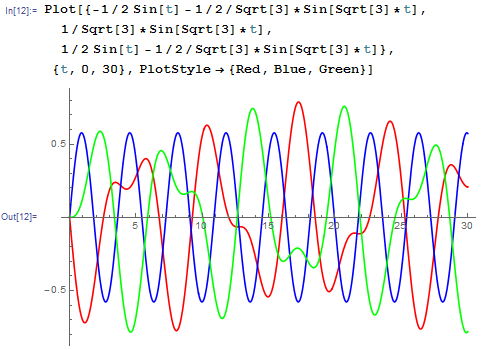
\includegraphics[width=11
    cm]{54.png}
    \caption{Figure for $v_1
    (t)=-\dfrac{1}{2}sint-\dfrac{1}{2\sqrt{3}}sin\sqrt{3}t,v_2=\dfrac{1}{\sqrt{3}}sin\sqrt{3}t,v_3(t)=\dfrac{1}{2}sint-\dfrac{1}{2\sqrt{3}}sin\sqrt{3}t$,red for $v_1(t)$, blue for $v_2$, green for $v_3$.}
\end{figure}

\begin{figure}[H]
    \centering
    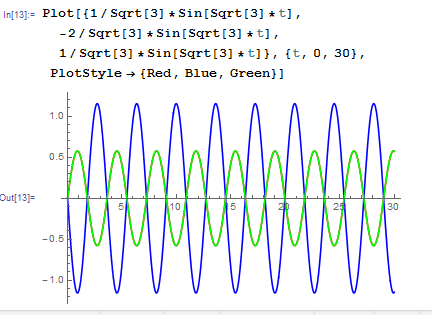
\includegraphics[width=11
    cm]{55.png}
    \caption{Figure for $v_1(t)=\dfrac{1}{\sqrt{3}}sin\sqrt{3}t,v_2=-\dfrac{2}{\sqrt{3}}sin\sqrt{3}t,v_3(t)=\dfrac{1}{\sqrt{3}}sin\sqrt{3}t$,red for $v_1(t)$, blue for $v_2$, green for $v_3$.}
\end{figure}


\begin{figure}[H]
    \centering
    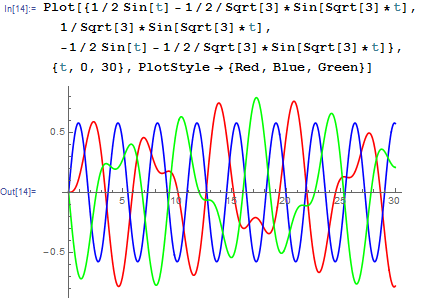
\includegraphics[width=11
    cm]{56.png}
    \caption{Figure for $v_3
    (t)=-\dfrac{1}{2}sint-\dfrac{1}{2\sqrt{3}}sin\sqrt{3}t,v_2=\dfrac{1}{\sqrt{3}}sin\sqrt{3}t,v_1(t)=\dfrac{1}{2}sint-\dfrac{1}{2\sqrt{3}}sin\sqrt{3}t$, red for $v_1(t)$, blue for $v_2$, green for $v_3$.}
\end{figure}

\begin{figure}[H]
    \centering
    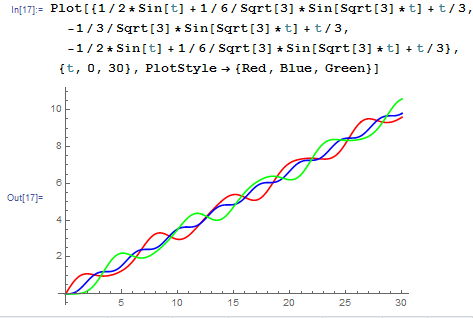
\includegraphics[width=11
    cm]{57.png}
    \caption{Figure for $d_1
    (t)=\dfrac{1}{2}sint+\dfrac{1}{6\sqrt{3}}sin\sqrt{3}t+\dfrac{t}{3},d_2=-\dfrac{1}{3\sqrt{3}}sin\sqrt{3}t+\dfrac{t}{3},d_3(t)=-\dfrac{1}{2}sint+\dfrac{1}{6\sqrt{3}}sin\sqrt{3}t+\dfrac{t}{3}$, red for $d_1(t)$, blue for $d_2$, green for $d_3$.}
\end{figure}


\begin{figure}[H]
    \centering
    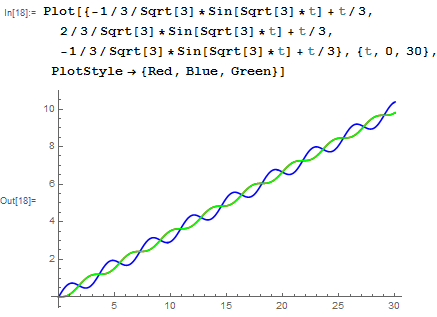
\includegraphics[width=11
    cm]{58.png}
    \caption{Figure for $d_1
    (t)=-\dfrac{1}{3\sqrt{3}}sin\sqrt{3}t+\dfrac{t}{3},d_2=\dfrac{2}{3\sqrt{3}}sin\sqrt{3}t+\dfrac{t}{3},d_3(t)=-\dfrac{1}{3\sqrt{3}}sin\sqrt{3}t+\dfrac{t}{3}$, red for $d_1(t)$, blue for $d_2$, green for $d_3$.}
\end{figure}

\begin{figure}[H]
    \centering
    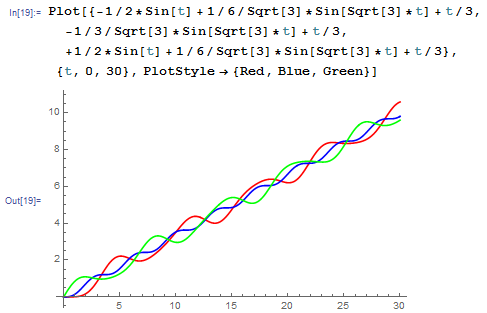
\includegraphics[width=13
    cm]{59.png}
    \caption{Figure for $d_3
    (t)=\dfrac{1}{2}sint+\dfrac{1}{6\sqrt{3}}sin\sqrt{3}t+\dfrac{t}{3},d_2=-\dfrac{1}{3\sqrt{3}}sin\sqrt{3}t+\dfrac{t}{3},d_1(t)=-\dfrac{1}{2}sint+\dfrac{1}{6\sqrt{3}}sin\sqrt{3}t+\dfrac{t}{3}$, red for $d_1(t)$, blue for $d_2$, green for $d_3$.}
\end{figure}

\begin{figure}[H]
    \centering
    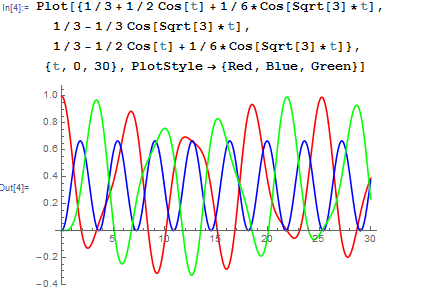
\includegraphics[width=11
    cm]{51.png}
    \caption{Figure for $d_1(t)=\dfrac{1}{3}+\dfrac{1}{2}cost+\dfrac{1}{6}cos\sqrt{3}t,d_2=\dfrac{1}{3}-\dfrac{1}{3}cos\sqrt{3}t,d_3(t)=\dfrac{1}{3}-\dfrac{1}{2}cost+\dfrac{1}{6}cos\sqrt{3}t$,red for $d_1(t)$, blue for $d_2$, green for $d_3$.}
\end{figure}

\begin{figure}[H]
    \centering
    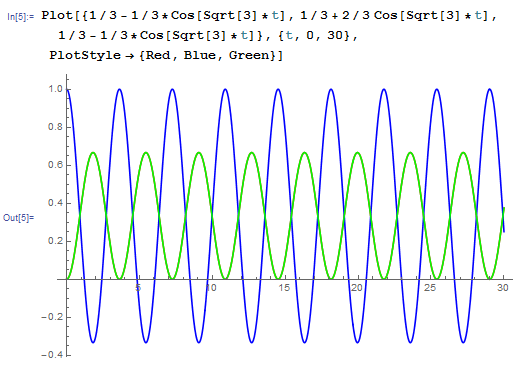
\includegraphics[width=11
    cm]{52.png}
    \caption{Figure for $d_1(t)=\dfrac{1}{3}-\dfrac{1}{3}cos\sqrt{3}t,d_2=\dfrac{1}{3}+\dfrac{1}{3}cos\sqrt{3}t,d_3(t)=\dfrac{1}{3}-\dfrac{1}{3}cos\sqrt{3}t$,red for $d_1(t)$, blue for $d_2$, green for $d_3$.}
\end{figure}

\begin{figure}[H]
    \centering
    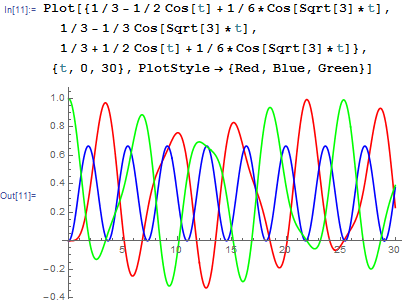
\includegraphics[width=11
    cm]{53.png}
    \caption{Figure for $d_3
    (t)=\dfrac{1}{3}+\dfrac{1}{2}cost+\dfrac{1}{6}cos\sqrt{3}t,d_2=\dfrac{1}{3}-\dfrac{1}{3}cos\sqrt{3}t,d_1(t)=\dfrac{1}{3}-\dfrac{1}{2}cost+\dfrac{1}{6}cos\sqrt{3}t$,red for $d_1(t)$, blue for $d_2$, green for $d_3$.}
\end{figure}
\subsection*{vi)}
$$\begin{pmatrix}
1\\
0\\
-1\\
2\\
0\\
0
\end{pmatrix}=\begin{pmatrix}
v(0)\\
d(0)
\end{pmatrix}=\Phi(0)C=\mathds{1}C=\begin{pmatrix}
c_1\\
c_2\\
c_3\\
c_4\\
c_5\\
c_6
\end{pmatrix}$$
So
\begin{align*}
d&=c_1d^{(1)}+c_2d^{(2)}+c_3d^{(3)}+c_4d^{(4)}+c_5d^{(5)}+c_6d^{(6)}=\begin{pmatrix}
cost+sint+\dfrac{1}{3}cos\sqrt{3}t\\
\dfrac{2}{3}-\dfrac{2}{3}cos\sqrt{3}t\\
-cost-sint+\dfrac{1}{3}cos\sqrt{3}t
\end{pmatrix}
\end{align*}
So
$$\begin{pmatrix}
x_1(t)\\
x_2(t)\\
x_3(t)
\end{pmatrix}=\begin{pmatrix}
d_1\\
d_2\\
d_3
\end{pmatrix}+\begin{pmatrix}
r_1\\
r_2\\
r_3
\end{pmatrix}=\begin{pmatrix}
cost+sint+\dfrac{1}{3}cos\sqrt{3}t+\dfrac{14}{3}\\
\dfrac{26}{3}-\dfrac{2}{3}cos\sqrt{3}t\\
-cost-sint+\dfrac{1}{3}cos\sqrt{3}t+\dfrac{38}{3}\\
\end{pmatrix}$$

\begin{figure}[H]
    \centering
    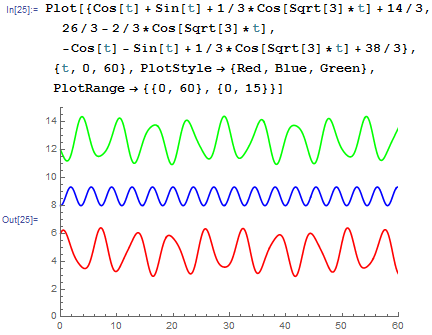
\includegraphics[width=14
    cm]{6.png}
    \caption{Figure for $x_1(t)=cost+sint+\dfrac{1}{3}cos\sqrt{3}t+\dfrac{14}{3},x_2(t)=\dfrac{26}{3}-\dfrac{2}{3}cos\sqrt{3}t,x_3(t)=
-cost-sint+\dfrac{1}{3}cos\sqrt{3}t+\dfrac{38}{3}$, red for $x_1(t)$, blue for $x_2(t)$, green for $x_3(t)$.}
\end{figure}

\section*{Exercise 4.4}
Since $A\in Mat(n\times n,\mathbb{C})$ and $A$ has $n$ eigenvalues, then $A$ is diagonlizable. Set $U\in  Mat(n\times n,\mathbb{C})$ satifies that
$U^{-1}AU=diag(\lambda_1, \cdots , \lambda_n)=:D$, then
\begin{align*}
detA=det\mathds{1}\cdot detA=det(U^{-1}U)\cdot detA=det(U^{-1}AU)=
\prod_{i=1}^n\lambda_i
\end{align*}

$$trA=tr(UDU^{-1})=tr(UU^{-1}D)=trD=\sum\limits_{i=1}^n\lambda_i$$

So $det(e^A)=det(Ue^DU^{-1})=det(e^D)=\prod_{i=1}^ne^{\lambda_i}=e^{\sum\limits_{i=1}^n\lambda_i}=e^{trA}$

To sum up, $detA=\prod_{i=1}^n\lambda_i,trA=\sum\limits_{i=1}^n\lambda_i,det(e^A)=e^{trA}$.
\section*{Exercise 4.5}
Since $\int sec\,t\,tan\,tdt=-sec\,t+C $ where $C$ is a constant and $y'''+y'=sec\,t\,tan\,t$, then 
$$y''+y=sec\,t+C$$
Since $y''(0)=y(0)=0$, $0+0=1+C$. So
$$y''+y=sec\,t-1$$
Set $x_1=y,x_2=\dot{x_1}$, then $x_1(0)=x_2(0)=0$ and
$$\begin{pmatrix}
\dot{x_1}\\
\dot{x_2}
\end{pmatrix}=\begin{pmatrix}
x_2\\
sect-1-x_1
\end{pmatrix}=\begin{pmatrix}
0&1\\
-1&0
\end{pmatrix}\begin{pmatrix}
x_1\\
x_2
\end{pmatrix}+\begin{pmatrix}
0\\
sect-1
\end{pmatrix}$$
Set $A=\begin{pmatrix}
0&1\\
-1&0
\end{pmatrix}$, then $det(A-\lambda\mathds{1})=0\Leftrightarrow \lambda=\pm i$. For $\lambda_1=i$, we find $u_1=\begin{pmatrix}
i\\
-1
\end{pmatrix}$, for $\lambda_2=-i$, we find $u_2=\begin{pmatrix}
i\\
1
\end{pmatrix}$. So the fundamental system is given by
$$\mathscr{F}=\lbrace e^{\lambda_1t}u_1,e^{\lambda_2t}u_2\rbrace=\lbrace\begin{pmatrix}
ie^{it}\\
-e^{it}
\end{pmatrix},\begin{pmatrix}
ie^{-it}\\
e^{-it}
\end{pmatrix}\rbrace$$

Set $\begin{pmatrix}
x_1\\
x_2
\end{pmatrix}=c_1(t)\begin{pmatrix}
ie^{it}\\
-e^{it}
\end{pmatrix}+c_2(t)\begin{pmatrix}
ie^{-it}\\
e^{-it}
\end{pmatrix}$. Then 
\begin{align*}
c_1(t)&=\int\dfrac{det\begin{pmatrix}
0&ie^{-it}\\
sect-1&e^{-it}
\end{pmatrix}}{det\begin{pmatrix}
ie^{it}&ie^{-it}\\
-e^{it}&e^{-it}
\end{pmatrix}}dt=\int 0.5(cost-isint-1+itant)dt\\
&=0.5(sint+icost-t+iln|cost|)
\end{align*}
\begin{align*}
c_2(t)&=\int\dfrac{det\begin{pmatrix}
ie^{it}&0\\
-e^{it}&sect-1
\end{pmatrix}}{det\begin{pmatrix}
ie^{it}&ie^{-it}\\
-e^{it}&e^{-it}
\end{pmatrix}}dt=\int 0.5(1-cost-isint+itant)dt\\
&=0.5(-sint+icost+t-iln|cost|)
\end{align*}
So $y=(0.5(sint+icost-t-iln|cost|)+C_1)ie^{it}+(0.5(-sint+icost+t+iln|cost|)+C_2)ie^{-it}$. Since $y'(0)=y(0)=0$, $C_1=C_2=-0.5i$.

To sum up, the solution to the initial value problem is $$y=-1+cost+tsint +cost\cdot ln|cost|$$
\section*{Exercise 4.6}
$$det(A-\lambda \mathds{1})=(-\lambda)(-b/a-\lambda)+b^2/(4a^2)=0\Leftrightarrow \lambda=-b/2a$$
\begin{align*}
(A+b/2a\cdot \mathds{1})v=0\Leftrightarrow
\begin{pmatrix}
b/(2a)&1\\
-b^2/(4a^2)&-b/(2a)
\end{pmatrix}\begin{pmatrix}
v_1\\
v_2
\end{pmatrix}=\begin{pmatrix}
0\\
0
\end{pmatrix}\Leftrightarrow v_2=-\dfrac{b}{2a}v_1
\end{align*}
So all the eigenvectors of $A$ are $k\begin{pmatrix}
-1\\
\dfrac{b}{2a}
\end{pmatrix},k\neq0$ and the eigenspace is $$V=\lbrace v:v=k\begin{pmatrix}
-1\\
\dfrac{b}{2a}
\end{pmatrix},k\in\mathbb{C}\rbrace$$
Now I want to show that $V\neq\mathbb{R}^2$ by proving that $u=\begin{pmatrix}
b\\
\dfrac{1}{2a}
\end{pmatrix}\notin V$.
This is because if $u\in V$, then $b=-k\wedge \dfrac{1}{2a}=\dfrac{bk}{2a}$, and therefore $b^2+1=0$. Since $b\in\mathbb{R}$, this is impossible. So $V\neq\mathbb{R}^2$.

To sum up, the matrix $A$ is not diagonalizable for any values of $a,b\in\mathbb{R}$.

\section*{Exercise 4.7}
\subsection*{i)}
Since $y_1(t)=t+1$ is a solution to the equation
$$y''-\dfrac{2(t+1)}{t^2+2t-1}y'+\dfrac{2}{t^2+2t-1}y=0$$
then we can set that $y_2(t)=v(t)(t+1)$, then
\begin{align*}
&y_2''-\dfrac{2(t+1)}{t^2+2t-1}y_2'+\dfrac{2}{t^2+2t-1}y_2=0\\
\Rightarrow&v''(t+1)+2v'-\dfrac{2(t+1)}{t^2+2t-1}(v'(t+1)+v)+\dfrac{2}{t^2+2t-1}v(t+1)=0\\
\Rightarrow&v''(t+1)=\dfrac{4}{t^2+2t-1}v'\\
\Rightarrow&\int\dfrac{1}{v'}d(v')=\int(\dfrac{1}{t+1-\sqrt{2}}-\dfrac{1}{t+1}+\dfrac{1}{t+\sqrt{2}+1}-\dfrac{1}{t+1})dt\\
\Rightarrow& lnv'=ln|t+1-\sqrt{2}|+ln|t+\sqrt{2}+1|-2ln|t+1|+C_1\\
\Rightarrow&v'=C_1\Big|\dfrac{t^2+2t-1}{t^2+2t+1}\Big|=C_1\Big|1-\dfrac{2}{(t+1)^2}\Big|\\
\Rightarrow&v(t)=\int C_1\Big|1-\dfrac{2}{(t+1)^2}\Big|dt=C_1\Big|t+\dfrac{2}{t+1}\Big|+C_2\\
\Rightarrow&y_2(t)=C_1|t^2+t+2|+C_2(t+1)
\end{align*}

So the general solution is $y(t)=C_1|t^2+t+2|+C_2(t+1) $, where $C_1,C_2\in\mathbb{R}$ are constant.

\subsection*{ii)}
Since $y_1(t)=\dfrac{sint}{\sqrt{t}}$ is a solution to the equation
$$t^2y''+ty'+(t^2-\dfrac{1}{4})y=0$$
then we can set that $y_2(t)=v(t)\dfrac{sint}{\sqrt{t}}$, then
\begin{align*}
&t^2y_2''+ty_2'+(t^2-\dfrac{1}{4})y_2=0\\
\Rightarrow&t^2y_1v''+(2t^2y'_1+ty_1)v'=0\\
\Rightarrow&v''=-\dfrac{2t^{3/2}cost}{t^{3/2}sint}v'=-(2cot\,t)v'\\
\Rightarrow&\int\dfrac{1}{v'}d(v')=-\int(2cot\,t)dt\\
\Rightarrow& lnv'=-2ln|sint|+C_1\\
\Rightarrow&v'=C_1\Big|\dfrac{1}{sin^2t}\Big|\\
\Rightarrow&v(t)=\int C_1\Big|\dfrac{1}{sin^2t}\Big|dt=C_1|cot\,t|+C_2\\
\Rightarrow&y_2(t)=C_1\dfrac{|cost|}{\sqrt{t}}+C_2\dfrac{sint}{\sqrt{t}}
\end{align*}

So the general solution is $y(t)=C_1\dfrac{|cost|}{\sqrt{t}}+C_2\dfrac{sint}{\sqrt{t}} $, where $C_1,C_2\in\mathbb{R}$ are constant.

\section*{Exercise 4.8}
\begin{figure}[H]
    \centering
    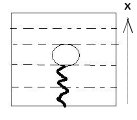
\includegraphics[width=8cm]{8.png}
\end{figure}

Set the position of mass is $x(t)$, the velocity and acceleration are $\dot{x(t)}=v(t),\ddot{x(t)}=a(t)$. The equilibrium is at $k(0-x)=mg\Rightarrow x=-10$. Then according to laws of Newton and Hooke, 
$$ma=k(x_0-x)-mg-\beta v$$
where $x_0$ is the initial length of the spring and therefore we can set it as 0. Then according to the question, 
$$x(0)=-10-1/4,v(0)=1,k=1,\beta=2,m=1$$
and use $g=10N/kg$, we can get
$$\ddot{x}+2\dot{x}+x+10=0,x(0)=-1/4,\dot{x}(0)=1$$

Set $x_1=x,x_2=\dot{x}$, then
$$\begin{pmatrix}
\dot{x_1}\\
\dot{x_2}
\end{pmatrix}=\begin{pmatrix}
x_2\\
-2x_2-x_1-10
\end{pmatrix}=\begin{pmatrix}
0&1\\
-1&-2
\end{pmatrix}\begin{pmatrix}
x_1\\
x_2
\end{pmatrix}-\begin{pmatrix}
0\\
10
\end{pmatrix}
$$

Set $A=\begin{pmatrix}
0&1\\
-1&-2
\end{pmatrix}$, $det(A-\lambda\mathds{1})=0\Leftrightarrow \lambda=-1$. For $\lambda=-1$, we find $u_1=\begin{pmatrix}
2\\
-2
\end{pmatrix}$. And from $(A+\mathds{1})u_2=u_1$, we find $u_2=\begin{pmatrix}
1\\
1
\end{pmatrix}$. Then set $U=(u_1,u_2)$ and we have
$$J=U^{-1}AU=\begin{pmatrix}
-1&1\\
0&-1
\end{pmatrix}$$
Then
$$e^{Jt}=\begin{pmatrix}
e^{-t}&0\\
0&e^{-t}
\end{pmatrix}\begin{pmatrix}
1&t\\
0&1
\end{pmatrix}=\begin{pmatrix}
e^{-t}&te^{-t}\\
0&e^{-t}
\end{pmatrix}$$
So $$Ue^{Jt}=\begin{pmatrix}
2e^{-t}&(2t+1)e^{-t}\\
-2e^{-t}&(1-2
t)e^{-t}
\end{pmatrix}$$

So the fundamental system is given by
$$\mathscr{F}=\lbrace\begin{pmatrix}
2e^{-t}\\
-2e^{-t}
\end{pmatrix},\begin{pmatrix}
(1+2t)e^{-t}\\
(1-2t)e^{-t}
\end{pmatrix}\rbrace$$


Set $\begin{pmatrix}
x_1\\
x_2
\end{pmatrix}=e^{-t}(c_1(t)\begin{pmatrix}
2\\
-2
\end{pmatrix}+c_2(t)\begin{pmatrix}
1+2t\\
1-2t
\end{pmatrix})$. Then 
\begin{align*}
c_1(t)=\int\dfrac{det\begin{pmatrix}
0&(1+2t)e^{-t}\\
-10&(1-2t)e^{-t}
\end{pmatrix}}{det\begin{pmatrix}
2e^{-t}&(1+2t)e^{-t}\\
-2e^{-t}&(1-2t)e^{-t}
\end{pmatrix}}dt=\int 2.5(1+2t)e^tdt=2.5(2t-1)e^t
\end{align*}
\begin{align*}
c_2(t)=\int\dfrac{det\begin{pmatrix}
2e^{-t}&0\\
-2e^{-t}&-10
\end{pmatrix}}{det\begin{pmatrix}
2e^{-t}&(1+2t)e^{-t}\\
-2e^{-t}&(1-2t)e^{-t}
\end{pmatrix}}dt=\int -5e^tdt=-5e^t
\end{align*}

So  $\begin{pmatrix}
x_1\\
x_2
\end{pmatrix}=e^{-t}((2.5(2t-1)e^t+C_1)\begin{pmatrix}
2\\
-2
\end{pmatrix}+(-5e^t+C_2)\begin{pmatrix}
1+2t\\
1-2t
\end{pmatrix})
$

So $x(t)=x_1(t)=-10+(2C_2t+2C_1+C_2)e^{-t},x_2(t)=(-2C_2t-2C_1+C_2)e^{-t}$. Since $x_1(0)=-10-1/4,x_2(0)=1$, $C_1=-5/16,C_2=3/8$. So
$$x(t)=-10+(\dfrac{3}{4}t-\dfrac{1}{4})e^{-t}$$

 We can see that $x(t)\leqslant -10 \Leftrightarrow 3/4t-1/4\leqslant 0\Leftrightarrow t\leqslant1/3$. So at $t=1/3$ the mass will over shoot its equilibrium and then it will never reach the equilibrium again. While since
 $$\underset{t\rightarrow\infty}{lim}x(t)=\underset{t\rightarrow\infty}{lim}-10+(\dfrac{3}{4}t-\dfrac{1}{4})e^{-t}=-10$$
so mass will overshoot its equilibrium position only once and then creep back to equilibrium.   

\section*{Exercise 4.9}
Set the position of mass is $x(t)$, the velocity and acceleration are $\dot{x(t)}=v(t),\ddot{x(t)}=a(t)$. Set the initial position of one side of the spring is $x=0$, then according to laws of Newton and Hooke, 
$$ma(t)+kx(t)=F(t)=Acos^3(\omega t)$$
Then according to the question, 
$$k=64,m=4$$
then we can get
$$4\ddot{x}+64x=Acos^3(\omega t) $$

Set $x_1=x,x_2=\dot{x}$, then
$$\begin{pmatrix}
\dot{x_1}\\
\dot{x_2}
\end{pmatrix}=\begin{pmatrix}
x_2\\
\dfrac{A}{4}cos^3(\omega t)-16x_1
\end{pmatrix}=\begin{pmatrix}
0&1\\
-16&0
\end{pmatrix}\begin{pmatrix}
x_1\\
x_2
\end{pmatrix}+\begin{pmatrix}
0\\
\dfrac{A}{4}cos^3(\omega t)
\end{pmatrix}
$$

Set $A=\begin{pmatrix}
0&1\\
-16&0
\end{pmatrix}$, $det(A-\lambda\mathds{1})=0\Leftrightarrow \lambda=\pm4i$. For $\lambda_1=-4i$, we find $u_1=\begin{pmatrix}
-1\\
4i
\end{pmatrix}$, for $\lambda_2=4i$, we find $u_2=\begin{pmatrix}
1\\
4i
\end{pmatrix}$.

So the fundamental system is given by
$$\mathscr{F}=\lbrace e^{\lambda_1t}u_1,e^{\lambda_2t}u_2\rbrace=\lbrace\begin{pmatrix}
-e^{-4it}\\
4ie^{-4it}
\end{pmatrix},\begin{pmatrix}
e^{4it}\\
4ie^{4it}
\end{pmatrix}\rbrace$$


Set $\begin{pmatrix}
x_1\\
x_2
\end{pmatrix}=c_1(t)\begin{pmatrix}
-e^{-4it}\\
4ie^{-4it}
\end{pmatrix}+c_2(t)\begin{pmatrix}
e^{4it}\\
4ie^{4it}
\end{pmatrix}$. Then 
\begin{align*}
c_1(t)&=\int\dfrac{det\begin{pmatrix}
0&e^{4it}\\
\dfrac{A}{4}cos^3(\omega t)&4ie^{4it}
\end{pmatrix}}{det\begin{pmatrix}
-e^{-4it}&e^{4it}\\
4ie^{-4it}&4ie^{4it}
\end{pmatrix}}dt=\int \dfrac{A}{128i}e^{4it}(cos(3\omega t)+3cos(\omega t))dt\\
&=\dfrac{Ae^{4it}}{128i}(\dfrac{1}{9\omega^2-16}(4icos(3\omega t)+sin(3\omega t))+\dfrac{3}{\omega^2-16}(4icos(\omega t)+sin(\omega t)))
\end{align*}
\begin{align*}
c_2(t)&=\int\dfrac{det\begin{pmatrix}
-e^{-4it}&0\\
4ie^{-4it}&\dfrac{A}{4}cos^3(\omega t)
\end{pmatrix}}{det\begin{pmatrix}
-e^{-4it}&e^{4it}\\
4ie^{-4it}&4ie^{4it}
\end{pmatrix}}dt=\int \dfrac{A}{128i}e^{-4it}(cos(3\omega t)+3cos(\omega t))dt\\
&=\dfrac{Ae^{-4it}}{128i}(\dfrac{1}{9\omega^2+16}(4icos(3\omega t)+sin(3\omega t))+\dfrac{3}{\omega^2+16}(4icos(\omega t)+sin(\omega t)))
\end{align*}

So
$$
x(t)=-\dfrac{Acos(3\omega t)}{81\omega^4-256}-\dfrac{Asin(3\omega t)}{4i(81\omega^4-256)}-\dfrac{3Acos(\omega t)}{\omega^4-256}-\dfrac{3Asin(\omega t)}{4i(\omega^4-256)}+C_2e^{4it}-C_1e^{-4it}
$$
So when $\omega^4=256$ or $81\omega^4-256=0$, i.e.$\omega=4$ or $\omega=4/3$, resonance will occur.

\section*{Exercise 4.10}
Set $x_1=y,x_2=\dot{x_1}$, then
$$\begin{pmatrix}
\dot{x_1}\\
\dot{x_2}
\end{pmatrix}=\begin{pmatrix}
x_2\\
-\dfrac{4}{3}\alpha x_2-\dfrac{2\alpha^2}{3}x_1
\end{pmatrix}=\begin{pmatrix}
0&1\\
-\dfrac{2\alpha^2}{3}&-\dfrac{4\alpha}{3}
\end{pmatrix}\begin{pmatrix}
x_1\\
x_2
\end{pmatrix}
,x_1(0)=0,x_2(0)=100$$

Set $A=\begin{pmatrix}
0&1\\
-\dfrac{2\alpha^2}{3}&-\dfrac{4\alpha}{3}
\end{pmatrix}$, $det(A-\lambda\mathds{1})=0\Leftrightarrow \lambda=(-\dfrac{2}{3}\pm\dfrac{\sqrt{2}}{3}i)\alpha$. For $\lambda_1=(-\dfrac{2}{3}+\dfrac{\sqrt{2}}{3}i)\alpha$, we find $u_1=\begin{pmatrix}
1\\
(-\dfrac{2}{3}+\dfrac{\sqrt{2}}{3}i)\alpha
\end{pmatrix}$, for $\lambda_2=-(\dfrac{2}{3}+\dfrac{\sqrt{2}}{3}i)\alpha$, we find $u_2=\begin{pmatrix}
1\\
-(\dfrac{2}{3}+\dfrac{\sqrt{2}}{3}i)\alpha
\end{pmatrix}$.

So the fundamental system is given by
$$\mathscr{F}=\lbrace e^{(-\dfrac{2}{3}+\dfrac{\sqrt{2}}{3}i)\alpha t}\begin{pmatrix}
1\\
(-\dfrac{2}{3}+\dfrac{\sqrt{2}}{3}i)\alpha
\end{pmatrix},e^{-(\dfrac{2}{3}+\dfrac{\sqrt{2}}{3}i)\alpha t}\begin{pmatrix}
1\\
-(\dfrac{2}{3}+\dfrac{\sqrt{2}}{3}i)\alpha
\end{pmatrix}\rbrace$$
Since $x_1(0)=0,x_2(0)=100$, then we can obtain that
$$x_1=-\dfrac{75\sqrt{2}}{\alpha}ie^{\lambda_1t}+\dfrac{75\sqrt{2}}{\alpha}ie^{\lambda_2t},
x_2=-\dfrac{75\sqrt{2}}{\alpha}i\lambda_1 e^{\lambda_1t}+\dfrac{75\sqrt{2}}{\alpha}i\lambda_2 e^{\lambda_2t}$$
So
\begin{align*}
y^2+(y')^2|_{t=1}&=Re(-\dfrac{11250}{\alpha^2}((1+\lambda_1^2)e^{2\lambda_1t}+(1+\lambda_2^2)e^{2\lambda_2t}))|_{t=1}\\
&=Re(-\dfrac{11250}{\alpha^2}((1+\lambda_1^2)e^{2\lambda_1}+(1+\lambda_2^2)e^{2\lambda_2}))\\
&=-\dfrac{11250}{\alpha^2}e^{-\frac{4}{3}\alpha}((2+\dfrac{4}{9}\alpha^2)cos\dfrac{2\sqrt{2}}{3}\alpha+\dfrac{8\sqrt{2}}{9}\alpha^2 sin\dfrac{2\sqrt{2}}{3}\alpha)
\end{align*}

So the $\alpha$ should satisfy that $$-\dfrac{11250}{\alpha^2}e^{-\frac{4}{3}\alpha}((2+\dfrac{4}{9}\alpha^2)cos\dfrac{2\sqrt{2}}{3}\alpha+\dfrac{8\sqrt{2}}{9}\alpha^2 sin\dfrac{2\sqrt{2}}{3}\alpha)\leqslant 0.01$$ 
\end{document}
